\chapter{Math Types and Coordinate Conventions}
\label{ch:math-conventions}
\label{ch:math-core-types}

CNA's math module carries the values that connect game code, content, effects, and renderers.
Its names follow XNA, but correct use depends on conventions that method names do not reveal:
row-vector matrix composition, a right-handed world basis, packed-color layout, interval
boundaries, and several incomplete geometric paths. This chapter explains those contracts.
Appendix~\ref{ch:api-quick-reference} is the compact API inventory; the module headers remain the
signature authority.

\section{Mental model}

Except for \cnaclass{BoundingFrustum}, the core types are C\texttt{++} value types with public
components or fields. Copying a \cnaclass{Vector3}, \cnaclass{Matrix}, \cnaclass{Rectangle}, or
\cnaclass{Color} copies its value; no framework identity or heap ownership is involved.
\cnaclass{BoundingFrustum} instead owns derived planes and corners behind its matrix property, so
it behaves more like a small object than a plain aggregate.

Most arithmetic families provide two spellings:

\begin{itemize}
  \item a value-returning form, such as \texttt{Vector3::Normalize(value)};
  \item an output-reference form with a trailing \texttt{result\&}, mirroring XNA's
        \texttt{ref}/\texttt{out} overloads.
\end{itemize}

They are separate public declarations. Do not assume the output-reference form is alias-safe:
some implementations write fields while still reading the input. The live
\cnaclass{Plane::Transform} defect later in this chapter is the consequential example.

\section{Common value surface}
\label{sec:shared-debug-surface}

The vectors, matrices, quaternions, planes, rays, integer geometry, bounding volumes, and
\cnaclass{CurveKey} expose equality and hashing; most also expose \texttt{ToString}. Hash return
types are not uniform: the port uses \texttt{int}, \texttt{intcs}, or
\texttt{std::size\_t} according to the type. Code that abstracts over these values should use
\texttt{auto} or its own normalized hash type.

Several types retain private debugger-display helpers, and the floating-point vectors,
\cnaclass{Matrix}, and \cnaclass{Quaternion} define \texttt{CheckForNaNs}. No external call site
or debugger visualizer was located at the pin. Vector checks are compiled unconditionally;
matrix and quaternion checks disappear under \texttt{NDEBUG}. This difference has no current
runtime effect because none of the helpers is called.

\section{Coordinate and composition contract}

Four rules carry into every graphics chapter:

\begin{enumerate}
  \item \cnaclass{Vector3::Forward} is $(0,0,-1)$ and
        \cnaclass{Vector3::Backward} is $(0,0,1)$: CNA follows XNA's right-handed world basis.
  \item CNA uses row-vector transforms. A position is conceptually multiplied on the left:
        $p' = pM$.
  \item Matrix products read in application order. With row vectors,
        \texttt{rotation * translation} rotates first and translates second.
  \item Perspective clip space needs four components. Preserve clip-space $W$ until clipping and
        the perspective divide have completed.
\end{enumerate}

This explains the standard world/view/projection product:

\[
  p_{\mathrm{clip}} = p_{\mathrm{object}}\,M_{\mathrm{world}}\,
                      M_{\mathrm{view}}\,M_{\mathrm{projection}} .
\]

The public depth convention is $[0,1]$. A renderer may translate that convention for its native
API, but application matrices and effects remain XNA-shaped.

\section{Vectors}

\cnaclass{Vector2}, \cnaclass{Vector3}, and \cnaclass{Vector4} provide public components,
zero/one and unit constants, arithmetic, dot products, distances, normalization, reflection,
clamping, and the XNA interpolation family. \cnaclass{Vector3} adds directions and
\texttt{Cross}; \cnaclass{Vector4} adds lower-dimensional transform inputs. Operations such as
\texttt{Lerp} are not clamped, so an amount outside $[0,1]$ extrapolates.

\subsection{Operation groups}
\label{sec:vector-full-reference}

\begin{center}
\small
\begin{tabular}{@{}p{0.25\textwidth}p{0.62\textwidth}@{}}
\toprule
\textbf{Group} & \textbf{Public families and boundary} \\
\midrule
Arithmetic & \texttt{Add}, \texttt{Subtract}, component/scalar \texttt{Multiply} and
  \texttt{Divide}, \texttt{Negate}, operators, \texttt{Min}, \texttt{Max}, and
  \texttt{Clamp}. \\
Measurement & \texttt{Length}, \texttt{LengthSquared}, \texttt{Distance},
  \texttt{DistanceSquared}, and \texttt{Dot}; \cnaclass{Vector3} adds \texttt{Cross}. \\
Interpolation & \texttt{Lerp}, \texttt{SmoothStep}, \texttt{Barycentric},
  \texttt{CatmullRom}, and \texttt{Hermite}. Amounts are caller-controlled. \\
Transforms & Matrix and quaternion \texttt{Transform}, plus array/range forms.
  \texttt{TransformNormal} omits translation and exists for \cnaclass{Vector2}/
  \cnaclass{Vector3}. \\
\bottomrule
\end{tabular}
\end{center}

Normalizing a zero vector divides by zero; CNA does not substitute a fallback direction. Validate
input when non-finite output would escape into gameplay or rendering.

\begin{lstlisting}
// Illustrative: move toward a target without overshooting it.
Vector2 toTarget = target - position;
const float distance = toTarget.Length();
if (distance > 0.0001f)
{
    toTarget.Normalize();
    position = position + toTarget *
        std::min(speed * deltaSeconds, distance);
}
\end{lstlisting}

Cross-product order sets the normal's sign. For a triangle $(a,b,c)$,
\texttt{Cross(b - a, c - a)} reverses if $b$ and $c$ are exchanged; the same winding choice
later controls face culling.

\subsection{Why Vector4 matters}

\texttt{Vector3::Transform(position, projection)} returns three components and therefore cannot
carry the projected $W$ needed by a software rasterizer or a manual clipping stage.
\cnaclass{Vector4} accepts a \cnaclass{Vector3} input directly:

\begin{lstlisting}
const Matrix combined = world * view * projection;
const Vector4 clip = Vector4::Transform(position, combined);
if (clip.W != 0.0f)
{
    const Vector3 ndc(
        clip.X / clip.W, clip.Y / clip.W, clip.Z / clip.W);
}
\end{lstlisting}

The Software renderer uses this four-component route before clipping and division. The snippet is
illustrative; production code must also handle the clip volume and the sign and magnitude of
\texttt{W}.

\section{Matrix}

\cnaclass{Matrix} stores \texttt{M11} through \texttt{M44}. Translation occupies the fourth
row, and direction properties expose the first three rows according to the right-handed basis.
The principal factory groups are translation, scale, rotations, quaternion conversion,
look-at/world, orthographic and perspective projections, billboards, planar shadow, and
reflection.

\subsection{Factory and arithmetic groups}
\label{sec:matrix-full-reference}
\label{sec:matrix-arithmetic}

\begin{center}
\small
\begin{tabular}{@{}p{0.25\textwidth}p{0.62\textwidth}@{}}
\toprule
\textbf{Purpose} & \textbf{Representative methods} \\
\midrule
Object transform & \texttt{CreateTranslation}, \texttt{CreateScale},
  \texttt{CreateRotationX/Y/Z}, \texttt{CreateFromAxisAngle},
  \texttt{CreateFromQuaternion}, \texttt{CreateFromYawPitchRoll}. \\
Camera/projection & \texttt{CreateLookAt}, \texttt{CreateWorld},
  \texttt{CreateOrthographic}, \texttt{CreateOrthographicOffCenter},
  \texttt{CreatePerspective*}. \\
Special geometry & \texttt{CreateBillboard}, \texttt{CreateConstrainedBillboard},
  \texttt{CreateShadow}, \texttt{CreateReflection}. \\
Algebra & \texttt{Add}, \texttt{Subtract}, matrix/scalar \texttt{Multiply} and
  \texttt{Divide}, \texttt{Negate}, \texttt{Invert}, \texttt{Transpose}, and
  component-wise \texttt{Lerp}. \\
\bottomrule
\end{tabular}
\end{center}

\texttt{Matrix::Lerp} interpolates all sixteen fields. It is not a substitute for decomposing a
transform and interpolating its rotation with \texttt{Quaternion::Slerp}. Likewise,
\texttt{Invert} does not report a singular input; callers that may receive degenerate transforms
need an independent validity check.

\texttt{Decompose(scale, rotation, translation)} returns \texttt{false} if any recovered axis
scale is near zero and sets rotation to identity. Scale and translation remain useful, but no
unique rotation can be extracted from the degenerate matrix.

\subsection{The ToColumnMajor bridge}

\texttt{CNAEXT Matrix::ToColumnMajor(float[16])} copies the sixteen fields in declaration order.
It does not numerically transpose the matrix. The bridge relies on the receiving shader API
interpreting those bytes as column-major storage: GLSL column $i$ corresponds to HLSL row $i$.
The dedicated identity test cannot distinguish a copy from a transpose, so renderer code and
non-identity tests remain the evidence for this convention.

\section{Quaternion}

\cnaclass{Quaternion} provides axis-angle, rotation-matrix, and yaw/pitch/roll construction;
normalization, conjugate and inverse; arithmetic; \texttt{Lerp}; and \texttt{Slerp}.

\subsection{Composition and interpolation}
\label{sec:quaternion-full-reference}

Quaternion multiplication is easy to read backwards: \texttt{q1 * q2} represents
\texttt{q2}'s rotation followed by \texttt{q1}'s. The explicitly named
\texttt{Quaternion::Concatenate(a, b)} instead promises $a$ followed by $b$. Use the named form
when operation order should be obvious at the call site.

\texttt{Lerp} chooses the short arc, linearly mixes components, and normalizes the result.
\texttt{Slerp} follows the sphere and gives uniform angular progress. For small turns the
difference is usually negligible; a long slow rotation can expose \texttt{Lerp}'s ease-in/ease-out
rate.

\begin{lstlisting}
Quaternion facing = Quaternion::CreateFromYawPitchRoll(
    0.0f, 0.0f, 0.0f);
const Quaternion target = Quaternion::CreateFromYawPitchRoll(
    MathHelper::PiOver2, 0.0f, 0.0f);

facing = Quaternion::Slerp(
    facing, target, std::min(1.0f, turnSpeed * deltaSeconds));
const Matrix orientation = Matrix::CreateFromQuaternion(facing);
\end{lstlisting}

The retained executable
\path{tools/cna-screenshot-infra/quaternion_vs_matrix_demo.cpp} compares a Z-axis matrix
rotation with the corresponding axis-angle quaternion route. At the pinned build used for the
artifact, the matrix components, transformed point, and rendered image agreed.

\section{Planes, rays, and bounding volumes}
\label{sec:bounding-volumes}

\cnaclass{Plane} stores a normal and distance; \texttt{DotCoordinate} includes the distance term
and classifies a point's side, whereas \texttt{DotNormal} tests a direction only.
\cnaclass{Ray} stores an origin and direction and returns \texttt{std::optional<float>} for
intersection distance. \cnaclass{BoundingBox}, \cnaclass{BoundingSphere}, and
\cnaclass{BoundingFrustum} expose containment and intersection families.

\subsection{Operational summary}
\label{sec:bounding-volumes-full-reference}

\begin{center}
\small
\begin{tabular}{@{}p{0.22\textwidth}p{0.34\textwidth}p{0.33\textwidth}@{}}
\toprule
\textbf{Type} & \textbf{Useful operations} & \textbf{Boundary} \\
\midrule
\cnaclass{Plane} & point/direction dot tests, normalization, volume intersection, matrix or
  quaternion transform & Matrix transform is defective at the pin; see below. \\
\cnaclass{Ray} & box, sphere, plane, and frustum intersection & Tolerances differ by shape;
  a zero direction is not a useful point query. \\
\cnaclass{BoundingBox} & create from points/sphere, merge, corners, containment/intersection &
  Touching and empty-input behavior follows individual implementations and exception types. \\
\cnaclass{BoundingSphere} & create from points/box, merge, transform, containment/intersection &
  A non-uniform transform remains a conservative sphere, not an ellipsoid. \\
\cnaclass{BoundingFrustum} & matrix-derived planes/corners, containment/intersection &
  Ray intersection currently checks origin containment rather than computing entry distance. \\
\bottomrule
\end{tabular}
\end{center}

\subsection{Current geometry defects}

\begin{limitationnote}
\textbf{Plane matrix transform.} The intended inverse-transpose path calls
\texttt{Matrix::Transpose(transformedMatrix, transformedMatrix)}. That output-reference overload
is not alias-safe: it overwrites fields that later reads still need. Identity and diagonal scale
hide the error; a translation or other nonsymmetric inverse exposes it. Avoid
\texttt{Plane::Transform(plane, matrix)} for nontrivial matrices at
\CnaRevisionShort. The quaternion overload does not use this path.
\end{limitationnote}

\begin{limitationnote}
\textbf{Frustum/ray intersection.} The pinned implementation classifies only the ray origin. An
origin outside the frustum returns \texttt{nullopt}, even when its direction enters the volume;
an origin inside returns zero. The remaining \texttt{Intersects} branch throws
\cnaclass{NotImplementedException}. This is not a general ray/frustum intersection algorithm.
\end{limitationnote}

Ray/box, ray/plane, and ray/sphere paths also use different parallel and behind-origin
tolerances. A zero-direction ray inside a box currently returns \texttt{nullopt}; validate and
normalize picking directions before querying several shapes.

\begin{lstlisting}
// Illustrative: choose the nearest successfully reported hit.
const SceneObject* nearest = nullptr;
float nearestDistance = std::numeric_limits<float>::max();
for (const SceneObject& candidate : candidates)
{
    if (const auto hit = pickRay.Intersects(candidate.GetBoundingBox());
        hit && *hit < nearestDistance)
    {
        nearestDistance = *hit;
        nearest = &candidate;
    }
}
\end{lstlisting}

\subsection{Transforming a bounding sphere}

\cnaclass{BoundingSphere::Transform} transforms the center and scales the radius by the largest
length of the matrix's three basis rows. Under a non-uniform scale $(2,3,4)$, a radius of $2$
becomes $8$. The result encloses the transformed ellipsoid, which is safe for broad-phase
culling but looser than an ellipsoid or oriented bound.

\section{Integer geometry and Color}

\cnaclass{Point} is the integer coordinate pair. \cnaclass{Rectangle} adds bounds, containment,
intersection/union, offset, and inflation. Rectangle right and bottom edges are exclusive for
point containment.

\texttt{Rectangle::IsEmpty} means exactly \texttt{X == Y == Width == Height == 0}. A zero-area
rectangle at another position is not empty by that property. Use
\texttt{Width > 0 \&\& Height > 0} when the question is whether a region has area.

\cnaclass{Color} stores byte channels and a packed \texttt{UInt32}. Its numeric packed form is
\texttt{AABBGGRR}; on little-endian systems the four packed bytes appear as RGBA. That statement
does not describe the layout of the polymorphic C\texttt{++} object itself, so renderer uploads
must use the supported conversion path instead of reinterpreting an array of \cnaclass{Color}.

\texttt{Color::FromNonPremultiplied} scales straight RGB channels by alpha for CNA's default
premultiplied-alpha blend path:

\begin{lstlisting}
const Color straight(200, 80, 40, 128);
const Color premultiplied =
    Color::FromNonPremultiplied(200, 80, 40, 128);
\end{lstlisting}

The type can hold either convention; the selected \cnaclass{BlendState} determines how the
channels are interpreted. Named color constants are generated API surface, not evidence about
blend behavior.

\section{MathHelper and degenerate inputs}

\cnaclass{MathHelper} collects angle constants, unit conversion, clamping, interpolation,
distance, wrapping, and epsilon comparison. \texttt{Lerp} is unclamped; \texttt{SmoothStep}
clamps its amount before applying the cubic curve. \texttt{WrapAngle} maps to a principal range
around zero.

Most lower-level math routines follow floating-point arithmetic instead of throwing on
degenerate inputs. Zero-vector normalization, singular inversion, coincident look-at inputs, and
invalid projection ranges can therefore yield infinities or NaNs. This policy is not uniform:
some factory methods validate selected range conditions while adjacent operations do not.
Validate at the boundary where bad values can affect gameplay, content, or a native API.

\section{Curves}

\cnaclass{Curve} evaluates an ordered \cnaclass{CurveKeyCollection}. Keys contain position,
value, incoming/outgoing tangents, and smooth/step continuity. \texttt{Add} inserts by ascending
position. \texttt{ComputeTangents} supports flat, linear, and smooth modes. Before and after the
key span, \texttt{Constant}, \texttt{Linear}, \texttt{Cycle}, \texttt{CycleOffset}, and
\texttt{Oscillate} choose clamping, extrapolation, wrapping, accumulated wrapping, or ping-pong
behavior.

\begin{lstlisting}
Curve height;
height.getKeysProperty().Add(CurveKey(0.0f, 10.0f));
height.getKeysProperty().Add(CurveKey(2.0f, 40.0f));
height.getKeysProperty().Add(CurveKey(4.0f, 10.0f));
height.ComputeTangents(CurveTangent::Smooth);
height.setPreLoopProperty(CurveLoopType::Constant);
height.setPostLoopProperty(CurveLoopType::Constant);

const float cameraHeight = height.Evaluate(elapsedSeconds);
\end{lstlisting}

This compiles against the public shape when the math headers and namespace aliases used by the
application are present; it is an illustrative fragment rather than a complete program.

\subsection{Current curve deviations}

Three source-level findings matter for nontrivial key positions:

\begin{itemize}
  \item Step evaluation compares the absolute query position with \texttt{1.0f}, not with the
        next key's position. Step intervals away from the canonical $[0,1]$ span can switch to the
        next value too early or too late.
  \item Post-loop linear extrapolation uses the \emph{first} key's outgoing tangent while
        extending from the last key.
  \item Smooth tangent computation uses materially different near-zero thresholds for incoming
        and outgoing spans, so duplicate or nearly duplicate positions can produce asymmetric
        tangents.
\end{itemize}

Both XNB and CNJ readers can construct curves. Their file-format and resolution contracts live in
Chapters~\ref{ch:xnb-type-readers} and~\ref{ch:cnj-format}; successful in-memory evaluation does
not establish either loading route.

\section{Compiled world/view/projection example}
\label{sec:worked-examples}

The retained source \path{tools/cna-screenshot-infra/math_rotation_demo.cpp} constructs a complete
game, builds a world/view/projection chain, applies \cnaclass{BasicEffect}, and draws a colored
triangle. Its central sequence is:

\begin{lstlisting}
const float angle = MathHelper::ToRadians(30.0f);
const Matrix world = Matrix::CreateRotationZ(angle) *
    Matrix::CreateTranslation(Vector3::Zero);
const Matrix view = Matrix::CreateLookAt(
    Vector3(0.0f, 0.0f, 3.0f), Vector3::Zero, Vector3::Up);
const Matrix projection = Matrix::CreatePerspectiveFieldOfView(
    MathHelper::PiOver4, 1.0f, 0.1f, 100.0f);

BasicEffect fx(dev);
fx.VertexColorEnabled = true;
fx.World = world;
fx.View = view;
fx.Projection = projection;
fx.Apply();
\end{lstlisting}

\begin{figure}[h]
\centering
\begin{figurealt}{Software-renderer matrix demonstration showing a colored three-dimensional object after world rotation, camera view, and projection transforms.}
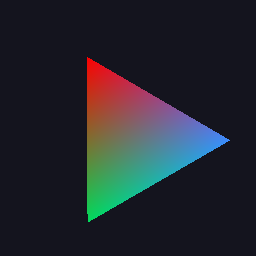
\includegraphics[width=0.4\textwidth]{images/ch07-matrix-rotation-software.png}
\end{figurealt}
\caption{Software-renderer output from the retained matrix demo. The image verifies the composed
rotation, view, projection, effect application, draw, and pixel path on the pinned configuration.}
\label{fig:ch07-matrix-rotation}
\end{figure}

\begin{evidencenote}
The image is a pixel artifact for one complete path, not a conformance oracle for every math
operation. The math test suite supplies analytic expectations at several tolerances, but this
edition located no captured XNA numeric corpus covering composition order, singular inputs,
corner ordering, or non-identity plane transforms. Porting tests should compare the original
program's observable results: projected positions, collision classifications, curve samples, or
captured reference values.
\end{evidencenote}

\section{Summary}

CNA's math API is broadly XNA-shaped, but its useful contract is the combination of value
semantics, row-vector composition, right-handed directions, and operation-specific edge cases.
Keep clip-space $W$, do not reinterpret polymorphic values as packed GPU bytes, validate
degenerate inputs, and avoid the current plane-matrix and frustum-ray paths where their missing
behavior matters.
